\uuid{ZxqW}
\exo7id{7713}
\titre{exo7 7713}
\auteur{mourougane}
\organisation{exo7}
\datecreate{2021-08-11}
\isIndication{false}
\isCorrection{true}
\chapitre{Sous-variété}
\sousChapitre{Sous-variété}
\module{Géométrie différentielle}
\niveau{L3}
\difficulte{}

\contenu{
\texte{
On considère la sphère de centre $0$ et de rayon $1$ de $\Rr^3$.
La projection stéréographique de centre le pôle Nord sur le plan de hauteur nulle (d'équation $z=0$)
conserve-t-elle les longueurs ? les angles ? les aires ?
}
\reponse{
On trouve en utilisant la relation $\vec{NP'}\parallel\vec{NP}$ 
que la projection stéréographique depuis le pôle nord sur le plan équatoriale est donnée par
$$\begin{array}{ccc}
  p : S^2&\to&\Rr^2\\\begin{pmatrix}x\\y\\z\end{pmatrix}&\mapsto&\begin{pmatrix}\frac{x}{1-z}\\ \frac{y}{1-z}\\0\end{pmatrix}
 \end{array}
$$

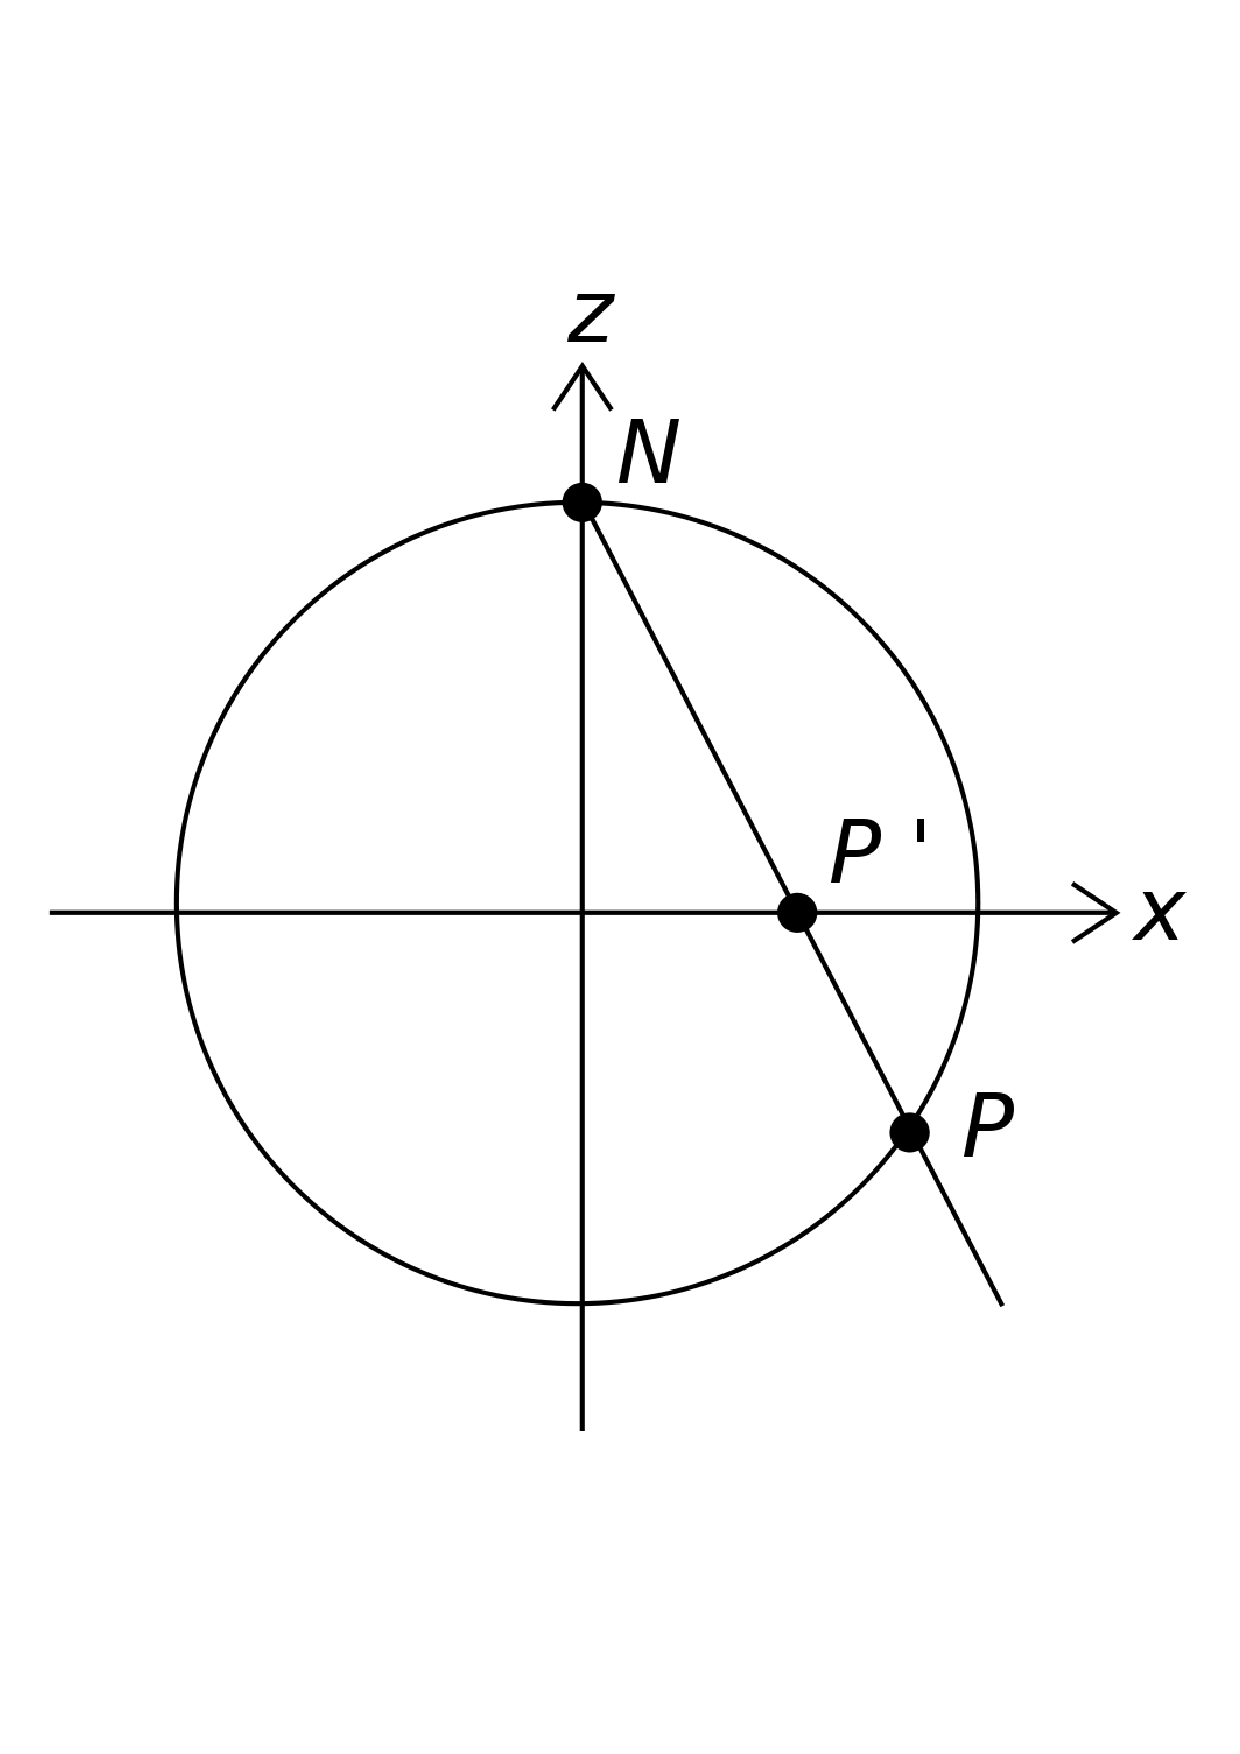
\includegraphics[scale=0.4]{images/pdf/ZxqW-1.pdf}

et la réciproque
$$\begin{array}{ccc}
F : \Rr^2&\to&S^2\\\begin{pmatrix}x'\\y'\end{pmatrix}&\mapsto&
\begin{pmatrix} \frac{2x'}{(x')^2+(y')^2+1}\\ \frac{2y'}{(x')^2+(y')^2+1}\\1-\frac{2}{(x')^2+(y')^2+1}\end{pmatrix}
\end{array}
$$
En particulier, la différentielle du paramétrage $F$ au point de paramètres $(0,0)$ est 
$$\begin{array}{cccc}
dF(0,0) : &T_{(0,0)}\Rr^2&\to&S_S^2\\ &\begin{pmatrix}X'\\Y'\end{pmatrix}&\mapsto&
\begin{pmatrix} 2X'\\ 2Y'\\0\end{pmatrix}
\end{array}
$$ n'est ni une isométrie, ni de déterminant $+/-1$.
La projection stéréographique ne conserve donc ni les longueurs, ni les aires.
Par contre, la différentielle du paramétrage $F$ au point de paramètres $(x',y')$ est 
$$\begin{array}{cccc}
dF(x',y') :& T_{(x',y')}\Rr^2&\to&TS^2\\ & \begin{pmatrix}X'\\Y'\end{pmatrix}&\mapsto&
\begin{pmatrix} 2\frac{-(x')^2+(y')^2+1}{((x')^2+(y')^2+1)^2}X'-4\frac{x'y'}{((x')^2+(y')^2+1)^2}Y'
\\ -4\frac{x'y'}{((x')^2+(y')^2+1)^2}X'+ 2\frac{(x')^2-(y')^2+1}{((x')^2+(y')^2+1)^2}Y'\\ 
4\frac{x'}{((x')^2+(y')^2+1)^2}X'+4\frac{y'}{((x')^2+(y')^2+1)^2}Y'\end{pmatrix}
\end{array}
$$
On vérifie alors que
$$\left\| dF(x',y')\begin{pmatrix}X'\\Y'\end{pmatrix}\right\|^2=\frac{4\left\|\begin{pmatrix}X'\\Y'\end{pmatrix}\right\|^2}{(x')^2+(y')^2+1}.$$
Donc, $dF(x',y')$ conserve les angles.
}
}
